\documentclass{ximera}
%\usepackage{todonotes}
%\usepackage{mathtools} %% Required for wide table Curl and Greens
%\usepackage{cuted} %% Required for wide table Curl and Greens
\newcommand{\todo}{}

\usepackage{esint} % for \oiint
\ifxake%%https://math.meta.stackexchange.com/questions/9973/how-do-you-render-a-closed-surface-double-integral
\renewcommand{\oiint}{{\large\bigcirc}\kern-1.56em\iint}
\fi


\graphicspath{
  {./}
  {ximeraTutorial/}
  {basicPhilosophy/}
  {functionsOfSeveralVariables/}
  {normalVectors/}
  {lagrangeMultipliers/}
  {vectorFields/}
  {greensTheorem/}
  {shapeOfThingsToCome/}
  {dotProducts/}
  {partialDerivativesAndTheGradientVector/}
  {../productAndQuotientRules/exercises/}
  {../normalVectors/exercisesParametricPlots/}
  {../continuityOfFunctionsOfSeveralVariables/exercises/}
  {../partialDerivativesAndTheGradientVector/exercises/}
  {../directionalDerivativeAndChainRule/exercises/}
  {../commonCoordinates/exercisesCylindricalCoordinates/}
  {../commonCoordinates/exercisesSphericalCoordinates/}
  {../greensTheorem/exercisesCurlAndLineIntegrals/}
  {../greensTheorem/exercisesDivergenceAndLineIntegrals/}
  {../shapeOfThingsToCome/exercisesDivergenceTheorem/}
  {../greensTheorem/}
  {../shapeOfThingsToCome/}
  {../separableDifferentialEquations/exercises/}
  {vectorFields/}
}

\newcommand{\mooculus}{\textsf{\textbf{MOOC}\textnormal{\textsf{ULUS}}}}

\usepackage{tkz-euclide}\usepackage{tikz}
\usepackage{tikz-cd}
\usetikzlibrary{arrows}
\tikzset{>=stealth,commutative diagrams/.cd,
  arrow style=tikz,diagrams={>=stealth}} %% cool arrow head
\tikzset{shorten <>/.style={ shorten >=#1, shorten <=#1 } } %% allows shorter vectors

\usetikzlibrary{backgrounds} %% for boxes around graphs
\usetikzlibrary{shapes,positioning}  %% Clouds and stars
\usetikzlibrary{matrix} %% for matrix
\usepgfplotslibrary{polar} %% for polar plots
\usepgfplotslibrary{fillbetween} %% to shade area between curves in TikZ
\usetkzobj{all}
\usepackage[makeroom]{cancel} %% for strike outs
%\usepackage{mathtools} %% for pretty underbrace % Breaks Ximera
%\usepackage{multicol}
\usepackage{pgffor} %% required for integral for loops



%% http://tex.stackexchange.com/questions/66490/drawing-a-tikz-arc-specifying-the-center
%% Draws beach ball
\tikzset{pics/carc/.style args={#1:#2:#3}{code={\draw[pic actions] (#1:#3) arc(#1:#2:#3);}}}



\usepackage{array}
\setlength{\extrarowheight}{+.1cm}
\newdimen\digitwidth
\settowidth\digitwidth{9}
\def\divrule#1#2{
\noalign{\moveright#1\digitwidth
\vbox{\hrule width#2\digitwidth}}}





\newcommand{\RR}{\mathbb R}
\newcommand{\R}{\mathbb R}
\newcommand{\N}{\mathbb N}
\newcommand{\Z}{\mathbb Z}

\newcommand{\sagemath}{\textsf{SageMath}}


%\renewcommand{\d}{\,d\!}
\renewcommand{\d}{\mathop{}\!d}
\newcommand{\dd}[2][]{\frac{\d #1}{\d #2}}
\newcommand{\pp}[2][]{\frac{\partial #1}{\partial #2}}
\renewcommand{\l}{\ell}
\newcommand{\ddx}{\frac{d}{\d x}}

\newcommand{\zeroOverZero}{\ensuremath{\boldsymbol{\tfrac{0}{0}}}}
\newcommand{\inftyOverInfty}{\ensuremath{\boldsymbol{\tfrac{\infty}{\infty}}}}
\newcommand{\zeroOverInfty}{\ensuremath{\boldsymbol{\tfrac{0}{\infty}}}}
\newcommand{\zeroTimesInfty}{\ensuremath{\small\boldsymbol{0\cdot \infty}}}
\newcommand{\inftyMinusInfty}{\ensuremath{\small\boldsymbol{\infty - \infty}}}
\newcommand{\oneToInfty}{\ensuremath{\boldsymbol{1^\infty}}}
\newcommand{\zeroToZero}{\ensuremath{\boldsymbol{0^0}}}
\newcommand{\inftyToZero}{\ensuremath{\boldsymbol{\infty^0}}}



\newcommand{\numOverZero}{\ensuremath{\boldsymbol{\tfrac{\#}{0}}}}
\newcommand{\dfn}{\textbf}
%\newcommand{\unit}{\,\mathrm}
\newcommand{\unit}{\mathop{}\!\mathrm}
\newcommand{\eval}[1]{\bigg[ #1 \bigg]}
\newcommand{\seq}[1]{\left( #1 \right)}
\renewcommand{\epsilon}{\varepsilon}
\renewcommand{\phi}{\varphi}


\renewcommand{\iff}{\Leftrightarrow}

\DeclareMathOperator{\arccot}{arccot}
\DeclareMathOperator{\arcsec}{arcsec}
\DeclareMathOperator{\arccsc}{arccsc}
\DeclareMathOperator{\si}{Si}
\DeclareMathOperator{\scal}{scal}
\DeclareMathOperator{\sign}{sign}


%% \newcommand{\tightoverset}[2]{% for arrow vec
%%   \mathop{#2}\limits^{\vbox to -.5ex{\kern-0.75ex\hbox{$#1$}\vss}}}
\newcommand{\arrowvec}[1]{{\overset{\rightharpoonup}{#1}}}
%\renewcommand{\vec}[1]{\arrowvec{\mathbf{#1}}}
\renewcommand{\vec}[1]{{\overset{\boldsymbol{\rightharpoonup}}{\mathbf{#1}}}\hspace{0in}}

\newcommand{\point}[1]{\left(#1\right)} %this allows \vector{ to be changed to \vector{ with a quick find and replace
\newcommand{\pt}[1]{\mathbf{#1}} %this allows \vec{ to be changed to \vec{ with a quick find and replace
\newcommand{\Lim}[2]{\lim_{\point{#1} \to \point{#2}}} %Bart, I changed this to point since I want to use it.  It runs through both of the exercise and exerciseE files in limits section, which is why it was in each document to start with.

\DeclareMathOperator{\proj}{\mathbf{proj}}
\newcommand{\veci}{{\boldsymbol{\hat{\imath}}}}
\newcommand{\vecj}{{\boldsymbol{\hat{\jmath}}}}
\newcommand{\veck}{{\boldsymbol{\hat{k}}}}
\newcommand{\vecl}{\vec{\boldsymbol{\l}}}
\newcommand{\uvec}[1]{\mathbf{\hat{#1}}}
\newcommand{\utan}{\mathbf{\hat{t}}}
\newcommand{\unormal}{\mathbf{\hat{n}}}
\newcommand{\ubinormal}{\mathbf{\hat{b}}}

\newcommand{\dotp}{\bullet}
\newcommand{\cross}{\boldsymbol\times}
\newcommand{\grad}{\boldsymbol\nabla}
\newcommand{\divergence}{\grad\dotp}
\newcommand{\curl}{\grad\cross}
%\DeclareMathOperator{\divergence}{divergence}
%\DeclareMathOperator{\curl}[1]{\grad\cross #1}
\newcommand{\lto}{\mathop{\longrightarrow\,}\limits}

\renewcommand{\bar}{\overline}

\colorlet{textColor}{black}
\colorlet{background}{white}
\colorlet{penColor}{blue!50!black} % Color of a curve in a plot
\colorlet{penColor2}{red!50!black}% Color of a curve in a plot
\colorlet{penColor3}{red!50!blue} % Color of a curve in a plot
\colorlet{penColor4}{green!50!black} % Color of a curve in a plot
\colorlet{penColor5}{orange!80!black} % Color of a curve in a plot
\colorlet{penColor6}{yellow!70!black} % Color of a curve in a plot
\colorlet{fill1}{penColor!20} % Color of fill in a plot
\colorlet{fill2}{penColor2!20} % Color of fill in a plot
\colorlet{fillp}{fill1} % Color of positive area
\colorlet{filln}{penColor2!20} % Color of negative area
\colorlet{fill3}{penColor3!20} % Fill
\colorlet{fill4}{penColor4!20} % Fill
\colorlet{fill5}{penColor5!20} % Fill
\colorlet{gridColor}{gray!50} % Color of grid in a plot

\newcommand{\surfaceColor}{violet}
\newcommand{\surfaceColorTwo}{redyellow}
\newcommand{\sliceColor}{greenyellow}




\pgfmathdeclarefunction{gauss}{2}{% gives gaussian
  \pgfmathparse{1/(#2*sqrt(2*pi))*exp(-((x-#1)^2)/(2*#2^2))}%
}


%%%%%%%%%%%%%
%% Vectors
%%%%%%%%%%%%%

%% Simple horiz vectors
\renewcommand{\vector}[1]{\left\langle #1\right\rangle}


%% %% Complex Horiz Vectors with angle brackets
%% \makeatletter
%% \renewcommand{\vector}[2][ , ]{\left\langle%
%%   \def\nextitem{\def\nextitem{#1}}%
%%   \@for \el:=#2\do{\nextitem\el}\right\rangle%
%% }
%% \makeatother

%% %% Vertical Vectors
%% \def\vector#1{\begin{bmatrix}\vecListA#1,,\end{bmatrix}}
%% \def\vecListA#1,{\if,#1,\else #1\cr \expandafter \vecListA \fi}

%%%%%%%%%%%%%
%% End of vectors
%%%%%%%%%%%%%

%\newcommand{\fullwidth}{}
%\newcommand{\normalwidth}{}



%% makes a snazzy t-chart for evaluating functions
%\newenvironment{tchart}{\rowcolors{2}{}{background!90!textColor}\array}{\endarray}

%%This is to help with formatting on future title pages.
\newenvironment{sectionOutcomes}{}{}



%% Flowchart stuff
%\tikzstyle{startstop} = [rectangle, rounded corners, minimum width=3cm, minimum height=1cm,text centered, draw=black]
%\tikzstyle{question} = [rectangle, minimum width=3cm, minimum height=1cm, text centered, draw=black]
%\tikzstyle{decision} = [trapezium, trapezium left angle=70, trapezium right angle=110, minimum width=3cm, minimum height=1cm, text centered, draw=black]
%\tikzstyle{question} = [rectangle, rounded corners, minimum width=3cm, minimum height=1cm,text centered, draw=black]
%\tikzstyle{process} = [rectangle, minimum width=3cm, minimum height=1cm, text centered, draw=black]
%\tikzstyle{decision} = [trapezium, trapezium left angle=70, trapezium right angle=110, minimum width=3cm, minimum height=1cm, text centered, draw=black]

\begin{document}


\begin{problem} \textbf{Compute} the following limit, or \textbf{explain} why the limit does not exist.
  \[
  \lim_{\vector{x,y}\to \vector{0,0}} \frac{2x y + xy^2}{x y}
  \]
  
  \vfill
\end{problem}

\textbf{For problems 2--4,} consider the following contour plot for a
  differentiable function $F : \R^2 \to \R$.  The $x$-axis is
  horizontal and the $y$-axis is vertical.  Assume nothing too
  complicated happens between the contour lines.
\begin{image}[6in]
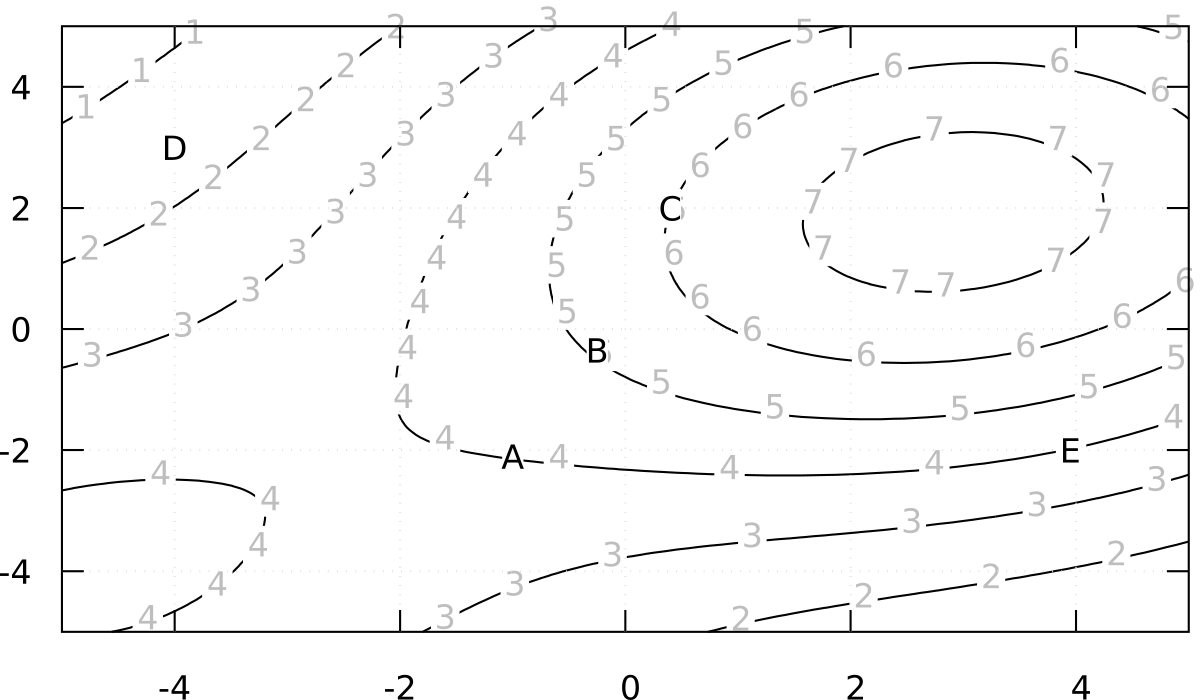
\includegraphics{contourPlot.png}
\end{image}

\begin{problem}
\textbf{On the plot above, draw} your best guess as to what the
\textbf{gradient vector} looks like at the point $A$.

\vfill

\end{problem}

\begin{problem}
  Do you think $\frac{\partial F}{\partial y}$ is \textbf{positive} or \textbf{negative} at the point $B$?  Why?


\vfill

\end{problem}




\begin{problem}
The point $D$ is at $(-4,3)$ and the point $E$ is at $(4,-2)$. Let
$\vec{v} = \grad F(-4,3)$ and let $\vec{w} = \grad F(4,-2)$.  Do you
think $|\vec{v}|$ or $|\vec{w}|$ is \textbf{larger?}  Why?


\vfill

\end{problem}
\textbf{Problem 5.} Suppose that $\vec{u}$ and $\vec{v}$ are nonzero three dimensional vectors.  \textbf{Show} that $\vec{u}$ and $\vec{v}$ are parallel if and only if $\vec{u} \cross \vec{v} = \vec{v} \cross \vec{u}$.

\vspace{80mm}

\textbf{Problem 6.}The curve $\mathcal{C}$ traced out by a vector-valued function $\vec{p}(s), 0 \leq s \leq 11$ and the points $P_0$ and $P_1$ associated to $\vec{p}(0)$ and $\vec{p}(11)$, respectively, are shown below.  Given that $\vec{p}(t)$ \underline{uses arclength as a parameter}, answer the following questions.  Make sure you \textbf{justify} your responses.


\begin{center}
\resizebox {6cm} {!} { 
    \begin{tikzpicture}
      \begin{axis}%
        [
	  xmin=-5,xmax=4.5,
          ymin=-4.5,ymax=4.5,
          xlabel=$x$,ylabel=$y$,
          axis lines=center,
          every axis y label/.style={at=(current axis.above origin),anchor=south},
          every axis x label/.style={at=(current axis.right of origin),anchor=west},
          clip=false,
	  grid =major,
          width=8cm,
          height=5cm,
          xtick={-4,-3,...,4},
          ytick={-5,-4,...,4},
	]
        \addplot[line join =bevel,penColor,ultra thick] coordinates{
          (-4,-4) (-4,0)(0,3) (2,3) 
        };
        \addplot[color=penColor,fill=penColor,only marks,mark=*] coordinates{(-4,-4)};  %% closed hole
        \addplot[color=penColor,fill=penColor,only marks,mark=*] coordinates{(2,3)};  %% closed hole
        %        \addplot[color=penColor,fill=penColor,only marks,mark=*] coordinates{(-1,-2)};  %% closed hole
        \node[penColor,right] at (axis cs: -4,-4.3) {\large $P_1$};
        \node[penColor,right] at (axis cs: 2,3) {\large $P_0$};
                
      \end{axis}
    \end{tikzpicture}}
\end{center}

\begin{itemize}
\item[A.] \textbf{Find} $s_0$ so $\vec{p}(s_0) = \vector{-4,-2}$.

\vspace{20mm}

\item[B.]  \textbf{Find} $\vec{p}(5)$.

\vspace{20mm}

\item[C.] \textbf{Find} $\vec{p}'(5)$.

\end{itemize}
\vspace{15mm}

\textbf{Problem 7.}\textbf{Multiselect}

\vspace{3mm}

\textbf{Directions:} A perfect response to this question is worth 10 points.  You will be penalized 2 points for each incorrect choice that you circle and each correct choice that you do not circle, but you cannot score below a 0.  Thus, the possible scores for this question are 0, 2, 4, 6, 8, or 10.  

\vspace{3mm}


\textbf{Problem}:  For the statements that follow, $\vec{u}$, $\vec{v}$, and $\vec{w}$ are nonzero three dimensional vectors.  The symbol $\dotp$ refers to the vector dot product, and $\cross$ refers to the vector cross product.  

\vspace{3mm}

\textbf{Circle} all of the following statements that \textbf{must} be true.  No justification is necessary.

\vspace{3mm}
\begin{itemize}
\item[I.] $|v|^2 = \vec{v} \dotp \vec{v}$ .   \\[3ex]
\item[II.] If $\proj_{\vec{u}}(\vec{v})$ is nonzero and $\vec{u}$ and $\proj_{\vec{u}}(\vec{v})$ are parallel, then $\vec{u}$ and $\vec{v}$ are parallel.  \\[3ex]
\item[III.] If $\vec{u}$ and$ \vec{v}$ are parallel, then $\proj_{\vec{w}}(\vec{u}) = \proj_{\vec{w}}(\vec{v})$ .     \\ [3 ex]
\item[IV.] $|v| \leq  \left|\proj_{\vec{u}}(\vec{v})\right|$.  \\[3ex]
\item[V.]  If $\vec{u}$ and $\vec{v}$ are orthogonal, then $\left|\vec{u}  \cross \vec{v} \right| = |u||v|$.   \\ [3 ex]
\item[VI.] $\vec{u} \dotp \left(\vec{v} \cross \vec{w}\right) = \left(\vec{u} \dotp \vec{v}\right) \cross \vec{w}$  \\[3ex]
%$\vec{u} \dotp \vec{v} = \vec{v} \dotp \vec{u}$ \\[ 3ex]
\item[VII.] $\vec{u} \dotp \left(\vec{u} \cross \vec{v}\right) = 0 $. \\[3ex]
\item[VIII.]  $\vec{u} = \proj_{\veci} \vec{u} + \proj_{\vecj} \vec{u}+\proj_{\veck} \vec{u}$ \\ [3 ex]
\item[IX.] If $\big| \vec{r} \, '(t) \big| = 1$ for all $t$, and $\vec{r}(0) =\vec{0}$, then $\big|\vec{r} (t)\big| = t$ for all $t$.\\[3ex]
\item[X.] If $\big| \vec{r} (t) \big| = 4$ for all $t$, then $\vec{r}' (t) = \vec{0}$.

\vspace{3mm}



\end{itemize}

\textbf{Problem 8.}Suppose that $\vec{r}(t) = \vector{t^3,4+3t^2}$ is defined for all $t$ and let $\mathcal{C}$ be the curve traced out by $\vec{r}(t)$ for $t\geq 0$.

\begin{enumerate}
\item[I.] \textbf{Find} all times $t$ at which $\vec{r}(t)$ and $\vec{r} \, ' (t)$ are orthogonal. 

\vspace{35mm}

\item[II.]  \textbf{Find} a vector $\vec{w}$ of length $17$ that is parallel to the tangent line to $\mathcal{C}$ at the point where $t=1$.  

\vspace{35mm}


\item[III.] \textbf{Explain} whether $\vec{r} (t)$ uses arclength as a parameter.  If it does not, find a vector-valued function $\vec{p}(s)$ that traces out $\mathcal{C}$ and uses arclength as a parameter.
\end{enumerate}


\textbf{Problem 9.} \textbf{Short Answer}

\begin{enumerate}
\item[I.]  Consider the vector-valued function $\vec{r}(t) = \vector{\frac{(t+4)^2}{e^t+3},\sqrt{1-2t},2+\ln(t+5)}$.  

\begin{itemize}
\item[A.]  \textbf{State} the domain of $\vec{r}(t)$.  No justification is necessary.

\vspace{35mm}

\item[B.]  \textbf{Explain} why the point $(0,3,2)$ lies on the curve traced out by $\vec{r}(t)$, then \textbf{find} a parametric representation of the tangent line to the curve traced out by $\vec{r}(t)$ at $(0,3,2)$.

\vspace{40mm}

\end{itemize}

\item[II.]  Suppose $\vec{u}=8\veci+5\vecj -10\veck$ and $\vec{v}= 2\veci+2\vecj-\veck$. 

\textbf{Find} a vector $\vec{P}$ parallel to $\vec{v}$ and a vector $\vec{N}$ orthogonal to $\vec{v}$ so that  $\vec{u} = \vec{P} + \vec{N}$.  

\vspace{65mm}

\textbf{Problem 10.}
\item[IV.] \textbf{Determine} whether the lines traced out by $\vec{r}_1(t) = \vector{2,1,0} t+\vector{-1,3,2}$ and $\vec{r}_2(T) = \vector{1,0,1} T+\vector{-1,4,1}$ are parallel, intersect each other, or are skew\footnote{Recall that two lines are \emph{skew} if they are nonparallel and nonintersecting.} and \textbf{explain} your response.  

\vspace{75mm}

\item[V.] \textbf{Explain} whether the conditional statement below is true.  


\end{enumerate}
\begin{quote}
``If $\uvec{v}$ is a unit vector in $\R^3$, then for every vector $\vec{u}$ in $\R^3$, $\vec{u} \dotp \uvec{v} = \scal_{\uvec{v}}{\vec{u}}$.'' 
\end{quote}

If it is false, give an explicit counterexample by finding vectors $\vec{u}$ and $\uvec{v}$ for which the hypothesis holds but the conclusion does not.

\newpage
\textbf{Problem 11 } Consider the vector-valued function $\vec{r}(t) =\vector{\cos(t),2\sin(t), \sin(t)}$, $0 \leq t \leq 2\pi$ and the plane defined by the equation $ax+3y-5z = 0$.

\begin{enumerate}
\item[I.]  If $a=1$, \textbf{determine} whether the curve traced out by $\vec{r}(t)$ intersects the plane and \textbf{give} the coordinates $(x,y,z)$ of all points of intersection.

\vspace{100mm}

\item[II.] \textbf{Find} a value for $a$ so the curve traced out by $\vec{r}(t)$ never intersects the plane or \textbf{explain} why no such $a$-value exists.

\end{enumerate}
\newpage
\textbf{Problem 12. }\textbf{Circle} the contour plot below that shows the level curves for the plane $z=x+y-1$.

\begin{center}
\resizebox {3.5cm} {!} { 
    \begin{tikzpicture}
      \begin{axis}%
        [
	  xmin=-1.5,xmax=1.5,
          ymin=-1.5,ymax=1.5,
          xlabel=$x$,ylabel=$y$,
          axis lines=center,
          every axis y label/.style={at=(current axis.above origin),anchor=south},
          every axis x label/.style={at=(current axis.right of origin),anchor=west},
          clip=false,
	  grid =major,
          width=8cm,
          height=5cm,
          xtick={-2,-1,...,2},
          ytick={-2,-1,1,2},
	]
            	\addplot [draw=penColor,very thick,smooth,domain=-1.5:-.5] {-2-x};
            	\addplot [draw=penColor,very thick,smooth,domain=-1.5:.5] {-1-x};
            	\addplot [draw=penColor,very thick,smooth,domain=-1.5:1.5] {-x};
            	\addplot [draw=penColor,very thick,smooth,domain=-.5:1.5] {1-x};
            	\addplot [draw=penColor,very thick,smooth,domain=.5:1.5] {2-x};
        %        \addplot[color=penColor,fill=penColor,only marks,mark=*] coordinates{(-1,-2)};  %% closed hole
                
      \end{axis}
    \end{tikzpicture}} 
    \qquad
\resizebox {3.5cm} {!} { 
    \begin{tikzpicture}
      \begin{axis}%
        [
	  xmin=-1.5,xmax=1.5,
          ymin=-1.5,ymax=1.5,
          xlabel=$x$,ylabel=$y$,
          axis lines=center,
          every axis y label/.style={at=(current axis.above origin),anchor=south},
          every axis x label/.style={at=(current axis.right of origin),anchor=west},
          clip=false,
	  grid =major,
          width=8cm,
          height=5cm,
          xtick={-2,-1,...,2},
          ytick={-2,-1,1,2},
	]
            	\addplot [draw=penColor,very thick,smooth,domain=-1.5:-.5] {2+x};
            	\addplot [draw=penColor,very thick,smooth,domain=-1.5:.5] {1+x};
            	\addplot [draw=penColor,very thick,smooth,domain=-1.5:1.5] {x};
            	\addplot [draw=penColor,very thick,smooth,domain=-.5:1.5] {-1+x};
            	\addplot [draw=penColor,very thick,smooth,domain=.5:1.5] {-2+x};
        %        \addplot[color=penColor,fill=penColor,only marks,mark=*] coordinates{(-1,-2)};  %% closed hole
                
      \end{axis}
    \end{tikzpicture}} 
\qquad
\resizebox {3.5cm} {!} { 
    \begin{tikzpicture}
      \begin{axis}%
        [
	  xmin=-1.5,xmax=1.5,
          ymin=-1.5,ymax=1.5,
          xlabel=$x$,ylabel=$y$,
          axis lines=center,
          every axis y label/.style={at=(current axis.above origin),anchor=south},
          every axis x label/.style={at=(current axis.right of origin),anchor=west},
          clip=false,
	  grid =major,
          width=8cm,
          height=5cm,
          xtick={-2,-1,...,2},
          ytick={-2,-1,1,2},
	]
            	\addplot [draw=penColor,very thick,smooth,domain=-1.5:-.75] {3+2*x};
            	\addplot [draw=penColor,very thick,smooth,domain=-1.5:0] {1.5+2*x};
            	\addplot [draw=penColor,very thick,smooth,domain=-.75:.75] {2*x};
            	\addplot [draw=penColor,very thick,smooth,domain=-0:1.5] {-1.5+2*x};
            	\addplot [draw=penColor,very thick,smooth,domain=.75:1.5] {-3+2*x};
        %        \addplot[color=penColor,fill=penColor,only marks,mark=*] coordinates{(-1,-2)};  %% closed hole
                
      \end{axis}
    \end{tikzpicture}} 
\qquad
\resizebox {3.5cm} {!} { 
    \begin{tikzpicture}
      \begin{axis}%
        [
	  xmin=-1.5,xmax=1.5,
          ymin=-1.5,ymax=1.5,
          xlabel=$x$,ylabel=$y$,
          axis lines=center,
          every axis y label/.style={at=(current axis.above origin),anchor=south},
          every axis x label/.style={at=(current axis.right of origin),anchor=west},
          clip=false,
	  grid =major,
          width=8cm,
          height=5cm,
          xtick={-2,-1,...,2},
          ytick={-2,-1,1,2},
	]
            	\addplot [draw=penColor,very thick,smooth,domain=-1.5:-.75] {-3-2*x};
            	\addplot [draw=penColor,very thick,smooth,domain=-1.5:0] {-1.5-2*x};
            	\addplot [draw=penColor,very thick,smooth,domain=-.75:.75] {-2*x};
            	\addplot [draw=penColor,very thick,smooth,domain=-0:1.5] {1.5-2*x};
            	\addplot [draw=penColor,very thick,smooth,domain=.75:1.5] {3-2*x};
        %        \addplot[color=penColor,fill=penColor,only marks,mark=*] coordinates{(-1,-2)};  %% closed hole
                
      \end{axis}
    \end{tikzpicture}} 




\end{center}

\textbf{Problem 13.} \textbf{State} the domain and range of $f(x,y) = \sqrt{4x^4+y^2+25}$.  No justification is necessary.

\vspace{35mm}



\vspace{50mm}
\newpage
\textbf{Problem 14.} (Limits) 

\textbf{Directions:}  For each part of the problem, \textbf{determine} whether the indicated limit exists or does not exist.  

\begin{itemize}
\item If a limit exists, \textbf{calculate} its value.  
\item If a limit does not exist, make sure that you provide clear justification to support your response.  

If your justification involves analyzing the function along different paths, you \textbf{must clearly state} the paths. Notation like $\Lim{(x,y)}{(a,b)^+} f(x,y)$ will be considered ambiguous and will result in a loss of points.
\end{itemize}

Parts I and II of this problem are unrelated.
\begin{enumerate}
\item[I.] $\Lim{(x,y)}{(0,0)} \frac{x^3y-xy^3}{x^4+y^4}$.

\vspace{25mm}

\item[II.] Let $f(x,y) =  \begin{cases} 2xy , & x+y \neq 5 \\[2 ex]  x^2y , & x+y = 5 \end{cases} $ . 

\item[A.] $\Lim{(x,y)}{(1,2)}f(x,y)$.

\vspace{25mm}

\item[B.] $\Lim{(x,y)}{(3,2)}f(x,y)$.


\end{enumerate}
 



\end{document}
